% KI-Übertragung in modernes Deutsch: Druckseiten 232--241.
% Principal PDF239--248; Google PDF243--252.
\begingroup
\clearpage
\noindent232\hfill\textsc{Trigonometrische Punktbestimmung.}\hfill\mbox{}\par\medskip
In Bezug auf einen zweiten Punkt bekannter Lage sollen $\varphi'$, $\alpha'$, $\beta'$, in Bezug auf einen dritten $\varphi''$, $\alpha''$, $\beta''$ usw. dasselbe bedeuten, was $\varphi$, $\alpha$, $\beta$ in Bezug auf den ersten bedeuten.

Sind die Winkelmessungen an dem zu bestimmenden Ort auf einmal mit einem Theodoliten ohne Repetition vorgenommen worden, indem bei unverrücktem Instrument das Fernrohr nacheinander auf die verschiedenen bekannten Punkte gerichtet wurde, so sollten, wenn $h$, $h'$, $h''$ usw. die dabei abgelesenen Winkel bezeichnen, die Ausdrücke
\[
\begin{gathered}
\varphi-h+\alpha\,\mathrm dx+\beta\,\mathrm dy\\
\varphi'-h'+\alpha'\mathrm dx+\beta'\mathrm dy\\
\varphi''-h''+\alpha''\mathrm dx+\beta''\mathrm dy\\
\text{usw.}
\end{gathered}
\]
durch Einsetzen der wahren Werte von $\mathrm dx$ und $\mathrm dy$ alle denselben Wert erhalten, wenn die Beobachtungen absolut genau wären. Setzte man also drei davon einander gleich, so würde man durch Elimination die Werte von $\mathrm dx$ und $\mathrm dy$ erhalten. Sind überhaupt nur drei bekannte Punkte beobachtet worden, so lässt sich auch nichts weiter tun. Ist ihre Anzahl größer, so werden die Fehler der Winkelmessungen am besten ausgeglichen, indem man alle obigen Ausdrücke addiert, die Summe durch die Anzahl dividiert, die Differenz zwischen diesem Quotienten und jedem einzelnen Ausdruck $=0$ setzt und diese Gleichungen nach der bekannten Vorschrift der Methode der kleinsten Quadrate behandelt.

Sind die Winkelmessungen dagegen unabhängig voneinander vorgenommen worden, so gibt jede von ihnen unmittelbar eine Gleichung zwischen den unbekannten Größen $\mathrm dx$ und $\mathrm dy$. Alle diese Gleichungen sind dann nach der Methode der kleinsten Quadrate zu kombinieren, wobei man nach Wunsch auch eine etwa ungleiche Zuverlässigkeit der Winkel berücksichtigen kann. Hätte man also z.\,B. den Winkel zwischen dem ersten und zweiten Punkt $=i$, zwischen dem zweiten und dritten $=i'$ usw. gefunden, stets von links nach rechts gerechnet, so hätte man die Gleichungen
\[
\begin{gathered}
\varphi'-\varphi-i+(\alpha'-\alpha)\mathrm dx+(\beta'-\beta)\mathrm dy=0\\
\varphi''-\varphi'-i'+(\alpha''-\alpha')\mathrm dx+(\beta''-\beta')\mathrm dy=0\\
\text{usw.}
\end{gathered}
\]

\clearpage
\noindent\mbox{}\hfill\textsc{Trigonometrische Punktbestimmung.}\hfill233\par\medskip
Haben diese Winkelmessungen die gleiche Zuverlässigkeit, so bildet man aus diesen Gleichungen zwei Normalgleichungen. Die erste erhält man, indem man die Gleichungen der Reihe nach mit den jeweiligen Koeffizienten von $\mathrm dx$ multipliziert, d.\,h. die erste mit $\alpha'-\alpha$, die zweite mit $\alpha''-\alpha'$ usw., und sie alle addiert. Die zweite erhält man auf dieselbe Weise durch Multiplikation mit den Koeffizienten von $\mathrm dy$ und anschließende Addition. Sind die Winkelmessungen dagegen von ungleicher Genauigkeit und beruht z.\,B. die erste auf $\mu$, die zweite auf $\mu'$ Repetitionen usw., so müssen die Gleichungen in beiden Fällen vor der Addition außerdem mit den jeweiligen Zahlen $\mu$, $\mu'$ usw. multipliziert werden. Aus den beiden so gefundenen Normalgleichungen werden dann $\mathrm dx$ und $\mathrm dy$ durch Elimination bestimmt. (Diese Vorschriften sind nur für diejenigen beigefügt, denen die Methode der kleinsten Quadrate noch unbekannt ist und die vielleicht auch noch daran erinnert werden müssen, dass bei diesen Multiplikationen die algebraischen Vorzeichen von $\alpha'-\alpha$ usw. sorgfältig beachtet werden müssen.) Schließlich bemerke ich noch, dass hierbei \textls[100]{nur} die Fehler der Winkelmessungen ausgeglichen werden sollen, da die Koordinaten der bekannten Punkte als \textls[100]{genau} angesehen werden.

Ich erläutere diese Vorschriften für den zweiten Fall noch anhand der mir von Ihnen mitgeteilten Winkelmessungen auf der Holkensbastion bei Kopenhagen, obwohl die zuletzt genannte Voraussetzung dabei, wie es scheint, nicht genau genug erfüllt ist. Bei so kleinen Entfernungen haben kleine Ungenauigkeiten von einigen Zehnteln eines Fußes in den gegebenen Koordinaten einen sehr viel größeren Einfluss als die Fehler in den Winkelmessungen. Man darf sich daher nicht wundern, dass nach bestmöglichem Ausgleich der Winkel Differenzen zurückbleiben, die weit über das hinausgehen, was bei den Beobachtungen der Winkel als möglich angenommen werden kann. Für den gegenwärtigen Zweck, zu dem nur ein Rechenbeispiel gegeben werden soll, kann dies jedoch gleichgültig sein.
\begin{center}
Winkel auf Holkensbastion\textsuperscript{*)}.
\end{center}
\begin{center}
\begin{tabular}{lrrr}
Friedrichsberg---Petri&$73^\circ$&$35'$&$22''{,}8$\\
Petri---Erlösersthurm&104&57&$33{,}0$
\end{tabular}
\end{center}
\vfill
\noindent\rule{4cm}{.4pt}\par
{\footnotesize *) Die Koordinaten der Punkte und die Winkel auf Holkensbastion beruhen beide auf den Messungen von Herrn Kapitän v.~\textsc{Caroc}.\quad $S$\textit{[chumacher].}\par}
\medskip\noindent{\small IX.}\hfill30\hspace*{2cm}

\clearpage
\noindent234\hfill\textsc{Trigonometrische Punktbestimmung.}\hfill\mbox{}\par\medskip
\begin{center}
\begin{tabular}{lrrr}
Erlösersthurm---Friedrichsberg&$181^\circ$&$27'$&$5''{,}0$\\
Friedrichsberg---Frauenthurm&80&37&$10{,}8$\\
Frauenthurm---Friedrichsthurm&101&11&$50{,}8$\\
Friedrichsthurm---Friedrichsberg&178&11&$1{,}5$.
\end{tabular}
\end{center}
\begin{center}
Koordinaten, von der Kopenhagener Sternwarte aus gerechnet, in Pariser Fuß.
\end{center}
\begin{center}
\begin{tabular}{lrr}
Petri&$+487{,}7$&$+1007{,}7$\\
Frauenthurm&$+710{,}0$&$+684{,}2$\\
Friedrichsberg&$+2430{,}6$&$+8335{,}0$\\
Erlösersthurm&$+2940{,}0$&$-3536{,}0$\\
Friedrichsthurm&$+3059{,}3$&$-2231{,}2$.
\end{tabular}
\end{center}
Als Näherungskoordinaten des Beobachtungsplatzes wurden angenommen:
\[
x=+2836{,}44,\qquad y=+444{,}33.
\]
Und damit ergaben sich die Azimute:
\[
\begin{array}{lrrr@{\;}l}
\text{Petri}&166^\circ&30'&42''{,}56&+19{,}92\mathrm dx+83{,}04\mathrm dy\\
\text{Frauenthurm}&173&33&50{,}54&+10{,}80\mathrm dx+95{,}78\mathrm dy\\
\text{Friedrichsberg}&92&56&39{,}46&+26{,}07\mathrm dx+\phantom01{,}34\mathrm dy\\
\text{Erlösersthurm}&271&29&25{,}38&-51{,}79\mathrm dx-\phantom01{,}35\mathrm dy\\
\text{Friedrichsthurm}&274&45&41{,}39&-76{,}56\mathrm dx-\phantom06{,}38\mathrm dy.
\end{array}
\]
Der berechnete Winkel Friedrichsberg---Petri ist daher
\[
73^\circ34'3''{,}10-6{,}15\mathrm dx+81{,}70\mathrm dy,
\]
was im Vergleich mit dem beobachteten Winkel die Gleichung
\[
-79{,}70-\phantom06{,}15\mathrm dx+\phantom081{,}70\mathrm dy=0
\]
ergibt. Ebenso erhält man die fünf anderen Gleichungen
\[
\begin{array}{r@{\;}r@{\;}r@{\;}l}
+69{,}82&-71{,}71\mathrm dx&-84{,}39\mathrm dy&=0\\
+9{,}08&+77{,}86\mathrm dx&+2{,}69\mathrm dy&=0\\
+0{,}28&-15{,}27\mathrm dx&+94{,}44\mathrm dy&=0\\
+0{,}05&-87{,}36\mathrm dx&-102{,}16\mathrm dy&=0\\
-3{,}43&+102{,}63\mathrm dx&+7{,}72\mathrm dy&=0.
\end{array}
\]
\clearpage
\noindent\mbox{}\hfill\textsc{Trigonometrische Punktbestimmung.}\hfill235\par\medskip
Aus der Verbindung dieser sechs Gleichungen erhält man, wenn man den Beobachtungen gleiche Zuverlässigkeit beimisst, die beiden Normalgleichungen
\[
\begin{aligned}
+29640\mathrm dx+14033\mathrm dy&=+\phantom04170\\
+14033\mathrm dx+33219\mathrm dy&=+12384,
\end{aligned}
\]
und daraus die Werte
\[
\mathrm dx=-0{,}04,\qquad\mathrm dy=+0{,}39,
\]
oder die verbesserten Koordinaten der Holkensbastion
\[
+2836{,}40\quad\text{und}\quad+444{,}72.
\]
Die nach dem Einsetzen dieser Werte von $\mathrm dx$ und $\mathrm dy$ zwischen den berechneten und beobachteten Winkeln verbleibenden Unterschiede sind noch viel zu groß, um den Messungen zugeschrieben werden zu können. Sie zeigen, wie oben bemerkt, dass die Koordinaten der bekannten Punkte nicht auf Zehntel eines Fußes zuverlässig waren, weshalb freilich auch die gefundene Verbesserung selbst diesmal etwas zweifelhaft bleibt.

Die dieser Rechnung zugrunde gelegten Näherungskoordinaten der Holkensbastion wurden mit der \textls[100]{direkten} Methode aus dem vierten und fünften der obigen Winkel berechnet. Obwohl diese direkte Methode als ein ziemlich erschöpfend behandelter Gegenstand anzusehen ist, führe ich sie der Vollständigkeit halber hier noch in der Form an, in der ich sie anzuwenden pflege.

Es seien $a$, $b$ die Koordinaten des ersten bekannten Punkts (man wählt ihn aus den drei bekannten nach Belieben). Die Koordinaten des zweiten seien in die Form
\[
a+R\cos E,\qquad b+R\sin E
\]
gebracht, und die des dritten in dieselbe:
\[
a+R'\cos E',\qquad b+R'\sin E'.
\]
Die gesuchten Koordinaten des Beobachtungspunkts bezeichne man durch
\[
a+\rho\cos\varepsilon,\qquad b+\rho\sin\varepsilon.
\]
Ferner sei der hier beobachtete Winkel zwischen dem ersten und zweiten
\vfill\noindent\hfill30\textsuperscript{$\ast$}\hspace*{2cm}

\clearpage
\noindent236\hfill\textsc{Trigonometrische Punktbestimmung.}\hfill\mbox{}\par\medskip
\noindent Punkt $=M$, der zwischen dem ersten und dritten $=M'$. Ich setze voraus, dass diese Winkel von links nach rechts genommen und, sofern sie dabei mehr als $180^\circ$ betragen haben, zunächst um $180^\circ$ vermindert worden sind. Das heißt, wenn ein in umgekehrter Reihenfolge genommener Winkel unter $180^\circ$ lag, wurde stattdessen sein Ergänzungswinkel zu $180^\circ$ genommen\textsuperscript{*)}. Ferner setze ich
\[
\begin{array}{rcl@{\qquad}rcl}
\frac R{\sin M}&=&n,&\frac{R'}{\sin M'}&=&n'\\[5pt]
E-M&=&N,&E'-M'&=&N'
\end{array}
\]
(wobei nötigenfalls vorher $360^\circ$ addiert wird).

Dies vorausgesetzt, hat man die beiden Gleichungen
\[
\rho=n\sin(\varepsilon-N),\qquad\rho=n'\sin(\varepsilon-N'),
\]
die, wenn man sie so schreibt,
\[
\frac1n=\frac1\rho\sin(\varepsilon-N),\qquad\frac1{n'}=\frac1\rho\sin(\varepsilon-N'),
\]
unter die Aufgabe Theor. Mot. C. C. p.~82 [**)] fallen. Eine der dort gegebenen Lösungen führt zu folgender Regel:

Ich nehme an, dass $n'$ größer als $n$ ist oder wenigstens ebenso groß. Das ist zulässig, da es beliebig ist, welchen Punkt man als den zweiten oder dritten betrachtet. Es sei
\[
\begin{gathered}
\frac n{n'}=\operatorname{tang}\zeta\\[5pt]
\frac{\operatorname{tang}\frac12(N'-N)}{\operatorname{tang}(45^\circ-\zeta)}=\operatorname{tang}\psi.
\end{gathered}
\]
Sodann wird
\[
\varepsilon=\tfrac12(N+N')+\psi,
\]
und nachdem $\varepsilon$ gefunden ist, wird $\rho$ nach einer der obigen Formeln oder besser nach beiden berechnet.

In unserem Beispiel haben wir den Frauenthurm als ersten, Friedrichsberg vorläufig als zweiten und den Friedrichsthurm als dritten Punkt betrachtet:
\vfill
\noindent\rule{4cm}{.4pt}\par
{\footnotesize
*) Damit sollen die folgenden Größen $n$, $n'$ stets positiv sein, sodass man weniger auf die algebraischen Vorzeichen achten muss.\par
[**) Band VII, Seite 100.]\par}

\clearpage
\noindent\mbox{}\hfill\textsc{Trigonometrische Punktbestimmung.}\hfill237\par\medskip
\[
\begin{array}{rcl@{\qquad}rcl}
a&=&+710{,}0&b&=&+684{,}2\\
E&=&77^\circ19'31''{,}91&E'&=&308^\circ51'45''{,}78\\
\log R&=&3{,}894\,4206&\log R'&=&3{,}573\,3549\\
M&=&99^\circ22'49''{,}20&M'&=&101^\circ11'50''{,}80\\
\multicolumn{3}{c}{\text{(gemäß obiger Anm.)}}&&&\\
N&=&337^\circ56'42''{,}71&N'&=&207^\circ39'54''{,}98\\
\log n&=&3{,}900\,2671&\log n'&=&3{,}581\,7019.
\end{array}
\]
Da hier $n>n'$ ist, vertauschen wir die Reihenfolge und setzen
\[
\begin{array}{rcl@{\qquad}rcl}
N&=&207^\circ39'54''{,}98&N'&=&337^\circ56'42''{,}71\\
\log n&=&3{,}581\,7019&\log n'&=&3{,}900\,2671.
\end{array}
\]
Danach ergeben sich ferner
\[
\zeta=25^\circ39'3''{,}49,\qquad
\psi=80^\circ45'31''{,}50,\qquad
\varepsilon=353^\circ33'50''{,}34
\]
und $\log\rho=3{,}330\,3996$, und für die Koordinaten der Holkensbastion ergeben sich $+2836{,}444$ und $+444{,}327$.
\vspace{1cm}
\begin{center}\rule{4cm}{.4pt}\end{center}

\clearpage
\noindent238\hfill\textsc{Nachlass.}\hfill\mbox{}\par
\vspace{1.5cm}
\begin{center}{\Large\textls[150]{NACHLASS.}}\end{center}
\bigskip
\begin{center}[7.]\\[5pt]
[Bestimmung der Lage des Punktes X durch Beobachtung der Winkel $\alpha$ und $\beta$ zwischen 3 gegebenen Punkten $A$, $B$, $C$.]
\end{center}
[Aus
\[
\frac{BA}{BX}.\frac{BX}{BC}.\frac{BC}{BA}=1
\]
folgt
\[
\frac{\sin XCB}{\sin BAX}=\frac{\sin C}{\sin A}=\frac{c\sin\beta}{a\sin\alpha}\,\bigg]
\]
\begin{center}
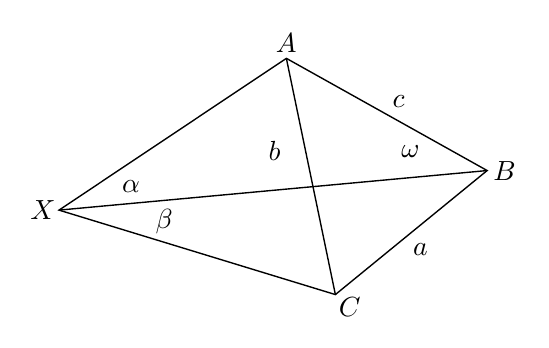
\begin{tikzpicture}[x=.75cm,y=.75cm,line width=.5pt]
\coordinate (X) at (0,0);
\coordinate (A) at (3.85,2.57);
\coordinate (B) at (7.25,.67);
\coordinate (C) at (4.68,-1.43);
\draw (X)--(A)--(B)--(C)--cycle;
\draw (X)--(B) (A)--(C);
\node[above,inner sep=2pt] at (A) {$A$};
\node[right,inner sep=2pt] at (B) {$B$};
\node[below right,inner sep=1pt] at (C) {$C$};
\node[left,inner sep=1pt] at (X) {$X$};
\node at (1.22,.40) {$\alpha$};
\node at (1.78,-.19) {$\beta$};
\node at (3.65,1.00) {$b$};
\node at (5.75,1.84) {$c$};
\node at (5.95,1.00) {$\omega$};
\node at (6.12,-.66) {$a$};
\end{tikzpicture}
\end{center}
[Setzt man
\[
\begin{gathered}
180^\circ-A=]\ \alpha+\omega=\lambda,\qquad [C=360^\circ-(A+\varepsilon),]\\
\alpha+\beta+B=\varepsilon\\[5pt]
\operatorname{tang}\varphi=\sqrt{\frac{c\sin\beta}{a\sin\alpha\cos\varepsilon}},
\end{gathered}
\]
dann ist
\[
\begin{gathered}
\operatorname{tang}\lambda=\operatorname{tang}\varepsilon\cos\varphi^2,\\
BX=\frac{c\sin\lambda}{\sin\alpha}.
\end{gathered}
\]
\clearpage
\noindent\mbox{}\hfill\textsc{Trigonometrische Punktbestimmung.}\hfill239\par\medskip
\begin{center}[8.]\\[5pt]Orientierung des Messtisches.\rlap{\hspace{.12em}\raisebox{1.15ex}{\scriptsize,}}\end{center}
Drei Orte $A$, $B$, $C$ sind auf dem M[ess]t[isch] durch $a$, $b$, $c$ dargestellt. Die geraden Linien $Aa$, $Bb$, $Cc$ schneiden einander in den Punkten $\alpha$, $\beta$, $\gamma$.

Die in $b$ auf $ab$ und in $\gamma$ auf $a\gamma$ errichteten Senkrechten schneiden einander in $e$. Die Senkrechten in $c$ auf $ac$ und in $\beta$ auf $a\beta$ schneiden einander in $f$. Man verbinde $e$ und $f$ und fälle darauf von $a$ aus das Lot $aM$. Damit ist $M$ der Standpunkt auf dem Messtisch.
\bigskip
\begin{center}[9.]\\[5pt]Aufgabe der praktischen Geometrie.\end{center}
$A$, $B$, $C$, $D$ sind vier Punkte in einer horizontalen Ebene. $B$, $C$, $D$ liegen auf einer Geraden und
\[
BC=CD.
\]
Es seien die Azimute der Linien
\[
\begin{array}{l@{\;}l}
DB\ .\ .\ .\ .&f\\
AB\ .\ .\ .\ .&f+g-\delta\\
AC\ .\ .\ .\ .&f+g-x\\
AD\ .\ .\ .\ .&f+g+\delta.
\end{array}
\]
\begin{center}
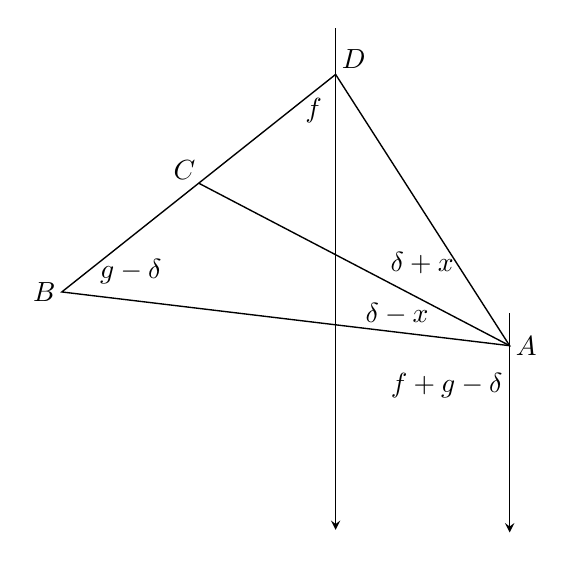
\begin{tikzpicture}[x=.65cm,y=.65cm,line width=.5pt]
\coordinate (B) at (0,0);
\coordinate (D) at (5.35,4.25);
\coordinate (C) at (2.675,2.125);
\coordinate (A) at (8.75,-1.05);
\draw (B)--(D)--(A)--cycle;
\draw (C)--(A);
\draw[->,>=stealth] (5.35,5.15)--(5.35,-4.65);
\draw[->,>=stealth] (8.75,-.42)--(8.75,-4.7);
\node[left,inner sep=2pt] at (B) {$B$};
\node[above left,inner sep=1pt] at (C) {$C$};
\node[above right,inner sep=2pt] at (D) {$D$};
\node[right,inner sep=2pt] at (A) {$A$};
\node at (1.35,.39) {$g-\delta$};
\node at (4.92,3.55) {$f$};
\node at (7.04,.57) {$\delta+x$};
\node at (6.55,-.44) {$\delta-x$};
\node at (7.52,-1.83) {$f+g-\delta$};
\end{tikzpicture}
\end{center}

\clearpage
\noindent240\hfill\textsc{Bemerkungen.}\hfill\mbox{}\par\medskip
\[
\bigg[\frac{AC}{BC}=\frac{AC}{CD}\quad\text{oder}\quad
\frac{\sin(g-\delta)}{\sin(\delta-x)}=\frac{\sin(g+\delta)}{\sin(\delta+x)}.\bigg]
\]
Sodann ist
\[
\begin{gathered}
\operatorname{tang}x=\frac{\operatorname{tang}\delta^2}{\operatorname{tang}g},\\[6pt]
\sin x=\frac{\sin\delta^2\cos(g-x)}{\sin g},
\end{gathered}
\]
oder näherungsweise
\[
x=206265''\sin\delta^2\operatorname{cotang}g.
\]
\bigskip
\begin{center}\rule{3cm}{.4pt}\\[6pt]\textsc{Bemerkungen.}\end{center}
\begingroup\footnotesize
Die Notizen [1] und [9], [3] und [4] sowie [8] wurden 3 verschiedenen Notizbüchern entnommen. [2] und [7] sind auf den letzten Seiten von Logarithmentafeln eingetragen. [5] stammt von einem Rechenblatt zur hannoverschen Gradmessung.

Die Formeln des Art.~[2], die auch in Art.~[3] verwendet werden, lassen sich wie folgt ableiten. Es seien $x$, $y$ die Koordinaten des zu bestimmenden Punktes, $x_0$, $y_0$ die Koordinaten seiner Näherungslage, $a$, $b$, $a'$, $b'$, $a''$, $b''$ die Koordinaten der Beobachtungsplätze und $r$, $r'$, $r''$ die Entfernungen dieser Plätze vom Punkt $(x_0,y_0)$. Dann erhält man durch Differenzieren der Gleichung
\[
\operatorname{tang}(A+\alpha)=\frac{y_0-b}{x_0-a},
\]
indem man $\mathrm dx_0=x-x_0$, $\mathrm dy_0=y-y_0$, $A+\alpha+\mathrm d(A+\alpha)=A+\delta A$ setzt, die Fehlergleichung:
\[
\delta A-\alpha=-\sin A.\frac{x-x_0}{r}+\cos A.\frac{y-y_0}{r}.
\]
Ebenso ergibt sich
\[
\delta A'-\alpha'=-\sin A'.\frac{x-x_0}{r'}+\cos A'.\frac{y-y_0}{r'}
\]
und
\[
\delta A''-\alpha''=-\sin A''.\frac{x-x_0}{r''}+\cos A''.\frac{y-y_0}{r''}.
\]
Eliminiert man $x-x_0$, $y-y_0$, so erhält man die Bedingungsgleichung:
\[
r\sin(A'-A'').(\delta A-\alpha)+r'\sin(A''-A).(\delta A'-\alpha')+r''\sin(A-A').(\delta A''-\alpha'')=0
\]
oder
\[
l.\delta A+l'.\delta A'+l''.\delta A''=l\alpha+l'\alpha'+l''\alpha''.
\]
Macht man nun mit Rücksicht hierauf
\[
g.\delta A^2+g'.\delta A'^2+g''.\delta A''^2\quad\text{zum Minimum},
\]
so wird
\par\endgroup

\clearpage
\noindent\mbox{}\hfill\textsc{Trigonometrische Punktbestimmung.}\hfill241\par\medskip
\begingroup\footnotesize
\[
\delta A=\frac{lk}{g},\qquad\delta A'=\frac{l'k}{g'},\qquad\delta A''=\frac{l''k}{g''};
\]
\[
k=\frac{l\alpha+l'\alpha'+l''\alpha''}{\dfrac{ll}{g}+\dfrac{l'l'}{g'}+\dfrac{l''l''}{g''}}.
\]
Danach ist
\[
y-b=(x-a)\operatorname{tang}(A+\delta A)=(x-a)\operatorname{tang}A+\frac{r.\delta A}{\cos A}
=(x-a)\operatorname{tang}A+\frac{rlk}{g\cos A}.
\]
In dem Zahlenbeispiel unter [3] sind einige kleine Fehler berichtigt worden. Dadurch weichen die hier erhaltenen Koordinatenwerte für York etwas von den im Koordinatenverzeichnis, Band IV, S.~436, angegebenen Werten ab.

Ebenso ist im Beispiel für das Vorwärtseinschneiden unter [5] ein kleines Versehen berichtigt worden. Die an den Festpunkten beobachteten Azimute und die Koordinaten sind auch in den »Abrissen u.\,s.\,w.«, Band IV, S.~454, 456 und 457, angegeben.

Zur Bestimmung von Nebenpunkten wandten \textsc{Gauss} und die ihm zugeteilten Offiziere gewöhnlich das Verfahren des Art.~[5] an. Die Rechnungen dafür führte jedoch fast ausschließlich \textsc{Gauss} in der angegebenen Weise aus. Im Arbeitsbericht für 1830 an das hannoversche Ministerium heißt es: »Bei der hiesigen trigonometrischen Vermessung habe ich bisher diesen Teil des Geschäfts [Auswertung der Messungen zur Gewinnung der Ergebnisse] ganz allein auf mich genommen. Meine Berichte über die Arbeiten von 1828 und 1829 geben eine Übersicht über den Umfang dessen, was in diesen Jahren geleistet wurde. Ohne hier auf ausführliche Einzelheiten einzugehen, muss ich doch erwähnen, dass mir die Auswertung nur dadurch möglich geworden ist, dass ich ihr meine \textls[100]{ganze} von meinen unmittelbaren Dienstgeschäften verbliebene Zeit gewidmet habe.« Und in dem am 8.~Februar 1838 erstatteten Bericht an das Ministerium sagt \textsc{Gauss}: »Zu einer trigonometrischen Messung sind zwei ganz verschiedene Arten von Arbeiten erforderlich: die Ausführung der Messungen an den betreffenden Orten im Feld und ihre Auswertung zur Gewinnung der Ergebnisse durch Kombination und Rechnung im Zimmer. Den zweiten Teil des Geschäfts habe ich bisher ganz auf mich selbst genommen.« Nur zwei Monate des Winters 1830/31 hat ihn sein Sohn, der Leutnant J.~\textsc{Gauss}, dabei unterstützt. In den letzten Jahren der hannoverschen Landesvermessung scheint auch Professor \textsc{Goldschmidt} geholfen zu haben. Einem von ihm ausgearbeiteten »geodätischen Calcül nach \textsc{Gauss}« aus dem Jahre 1835, der eine »kurze Darstellung nach privaten Mitteilungen von \textsc{Gauss}« bieten will, sind die nachstehenden Ausführungen entnommen:

»Bei der Festlegung der Nebenpunkte fangen wir damit an, diejenigen zu bestimmen, die sich allein aus den Punkten der Hauptdreiecke \textls[100]{genau} bestimmen lassen, sodass 1) die Richtungen sich nicht unter zu spitzen Winkeln schneiden und 2) man gewiss ist, dass die angeführten Azimute sich wirklich auf den fraglichen Punkt beziehen, da bei ausgedehnten Arbeiten leider nur zu häufig Namen verwechselt werden. Hat man den Punkt jedoch aus mehr als 2 Hauptpunkten bestimmt oder auf dem Punkt selbst gemessen, so kann eine solche Verwechslung kaum vorkommen. So legt man nun diese Nebenpunkte fest, indem man für genaue Ergebnisse sowohl alle Punkte der Hauptdreiecke als auch die nach und von anderen bereits bestimmten Nebenpunkten gemachten Schnitte heranzieht. Dabei entstehen 3 unbekannte Größen, die Koordinaten des Punkts und die dortige Orientierung. Man berechnet diese Elemente nun auch für die übrigen Nebenpunkte. Sollte es später für ratsam gehalten werden, neue Nebenpunkte einzuführen, weil es bei der anfänglichen Planung vielleicht übersehen wurde, dass ihre Einführung ratsam wäre, so braucht man sich doch nicht zu denjenigen Stationen zu begeben, von denen aus die neuen
\par\endgroup
\vfill\noindent{\small IX.}\hfill31\hspace*{2cm}
\endgroup
% Continues on printed 242 with "Punkte geschnitten werden könnten".
